
\documentclass[12pt,a4paper]{article} 

\usepackage{float,times,graphicx,mathtools}
\usepackage{amsmath}
\usepackage{amsfonts}
\usepackage{amssymb}
\usepackage{latexsym}
\usepackage{epsfig}
\usepackage{graphicx}
\usepackage{caption}
\usepackage{subcaption}
\usepackage{color}
\usepackage{pdfpages}
\usepackage{natbib}
\usepackage[space]{grffile}
\usepackage{wrapfig}
\usepackage{subcaption}
\usepackage{url}
\usepackage{bbm}
\usepackage{tikzsymbols}

\DeclareMathOperator{\logit}{logit}
\DeclareMathOperator{\tr}{tr}
\bibpunct[, ]{(}{)}{;}{a}{,}{,}
\graphicspath{{../}}  
\addtolength{\oddsidemargin}{-1in}
	\addtolength{\evensidemargin}{-1in}
	\addtolength{\textwidth}{1.75in}
	\addtolength{\topmargin}{-1.3in}
	\addtolength{\textheight}{2in}
\date{\vspace{-5ex}}
\begin{document}

\begin{itemize}
\item Fitted the LogQuad model to DHS data only in a few countries with relatively low HIV prevalence, and Zimbabwe and Zambia (just to see how badly the LQ model fits to high HIV countries), using IGME estimates for $h$
\item For females in countries with relatively low HIV, the LQ model generally suffices to describe the mortality schedule within the age range with DHS data (fiited to 15-49) and the estimated $h$ coincides with the IGME estimates
\item For males, the estimated $h$ differ from the IGME estimates in most cases, except for Niger (or Senegal) where HIV is very low
\item[*] LQ model fitted to DHS data in 5x5 grid at ages 15-49 vs Spline fitted to DHS data in 1x1 at ages 10-65 since 1990
\end{itemize}

\newpage
\section*{\centering Males}
\begin{figure}[H]
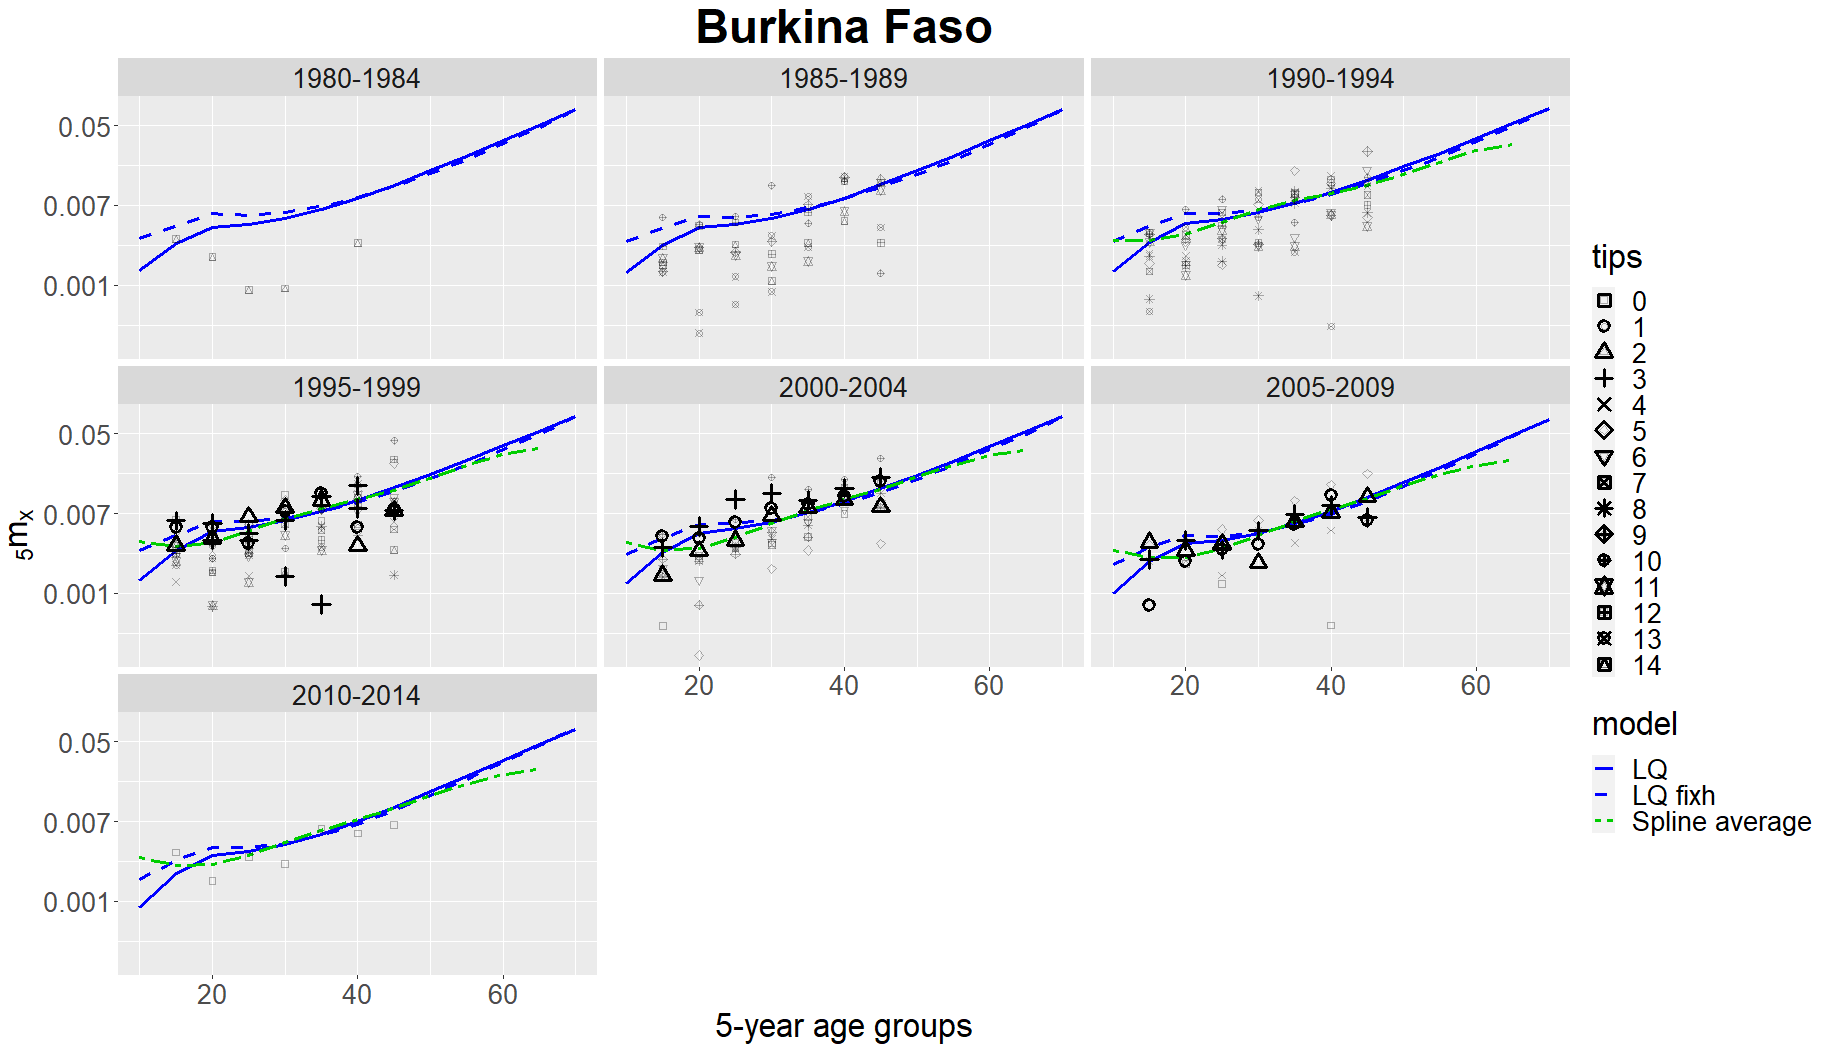
\includegraphics[width = \linewidth]{Burkina Faso/8/burkina faso males.png}
\end{figure}
\begin{figure}[H]
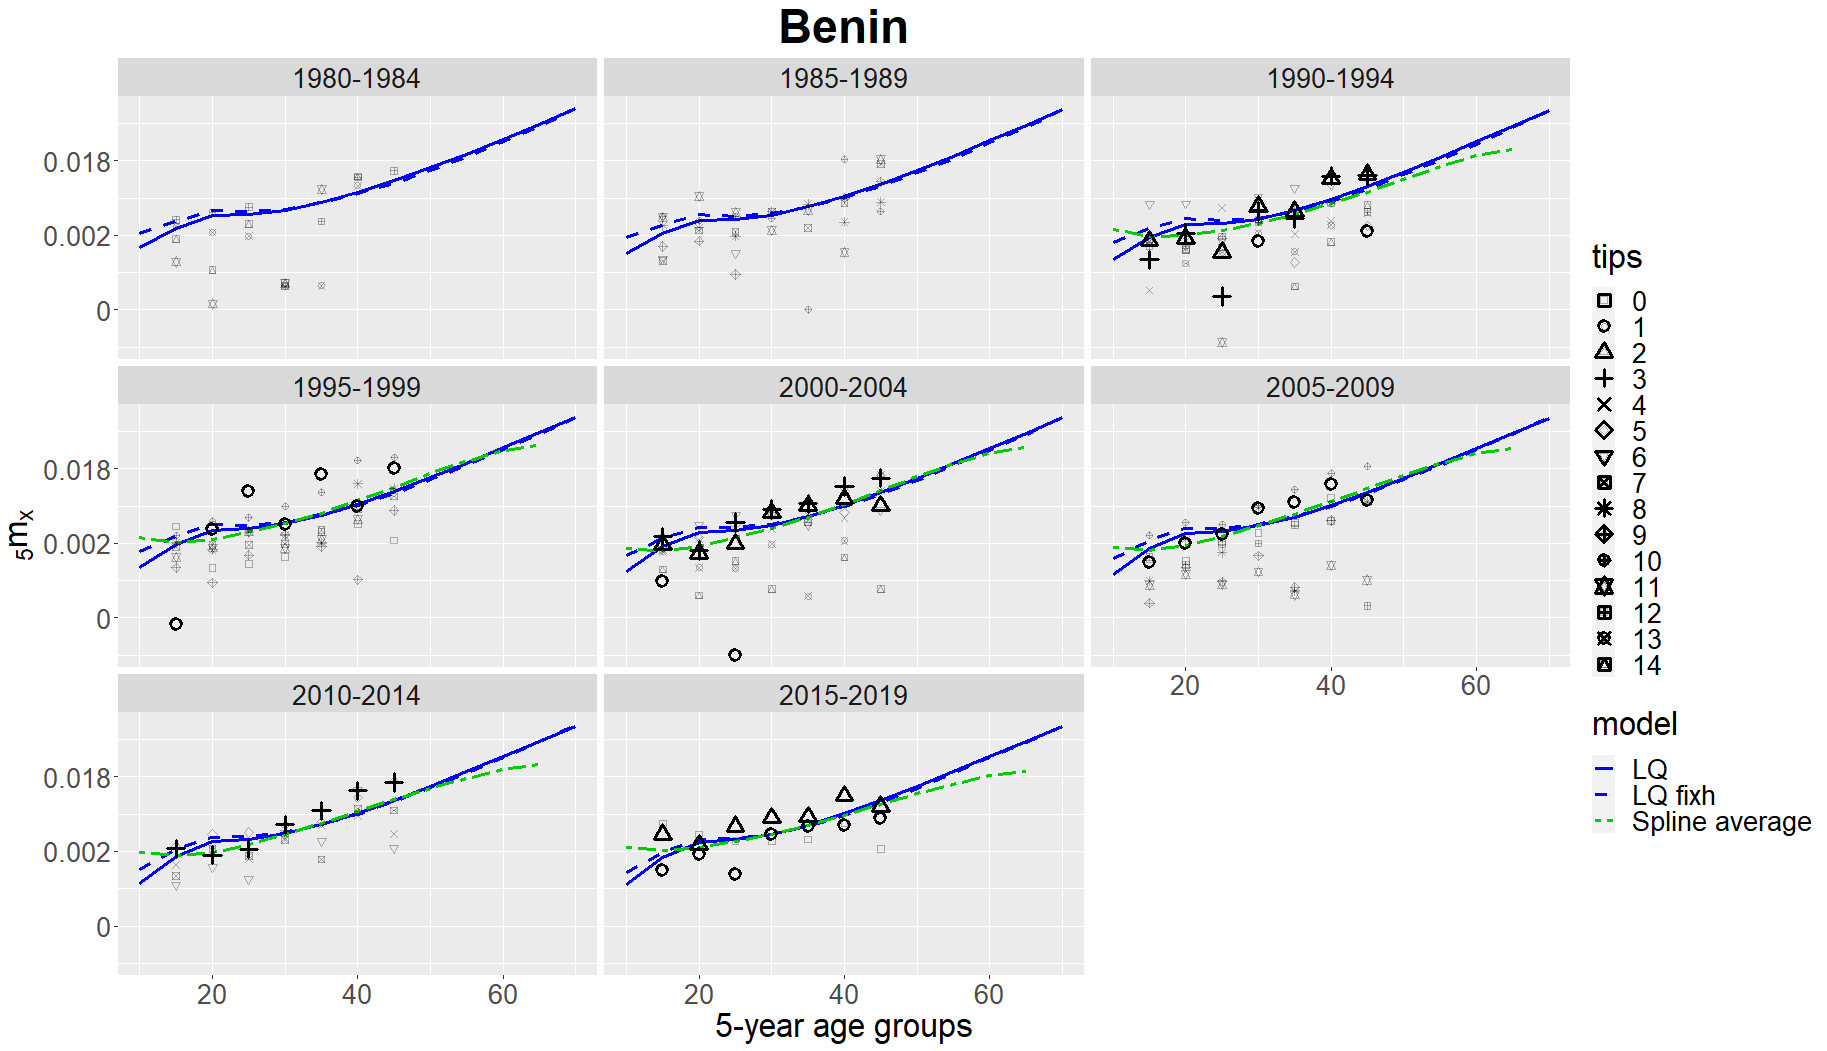
\includegraphics[width = \linewidth]{Burkina Faso/8/benin males.png}
\end{figure}

\newpage
\section*{\centering Males}
\begin{figure}[H]
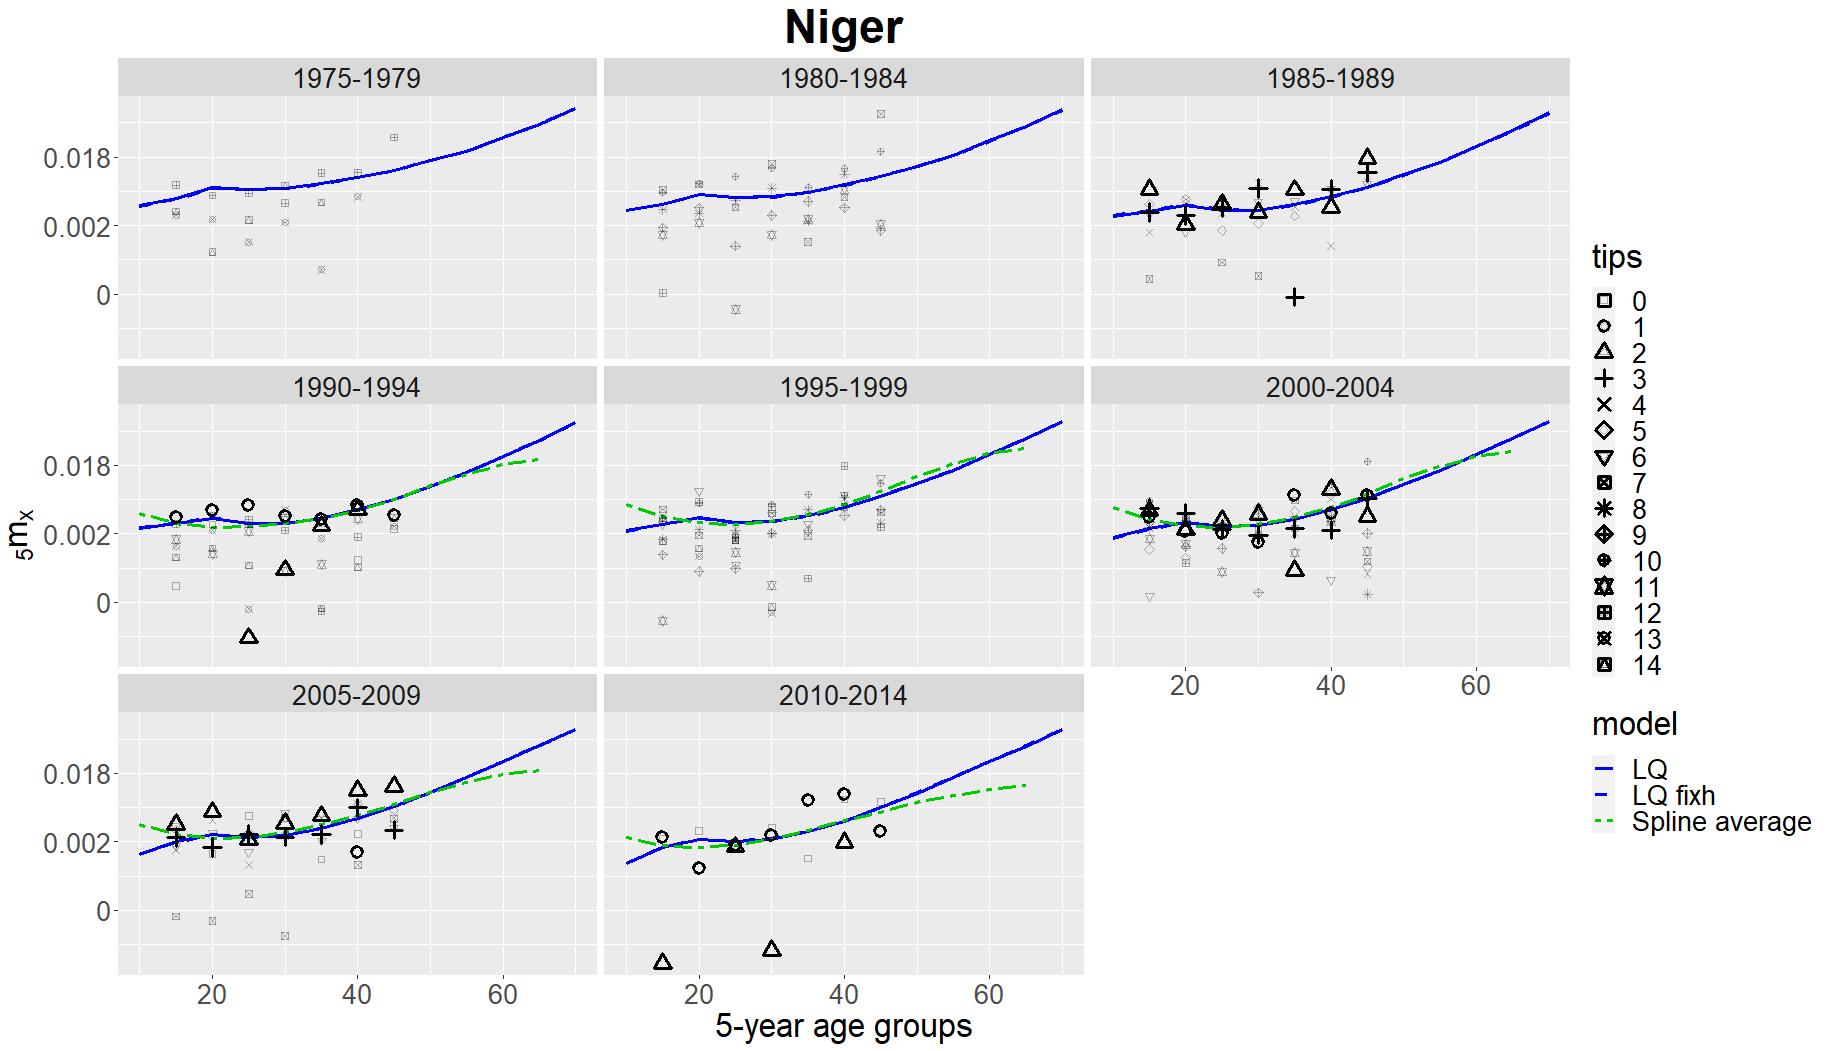
\includegraphics[width = \linewidth]{Burkina Faso/8/niger males.png}
\end{figure}
\begin{figure}[H]
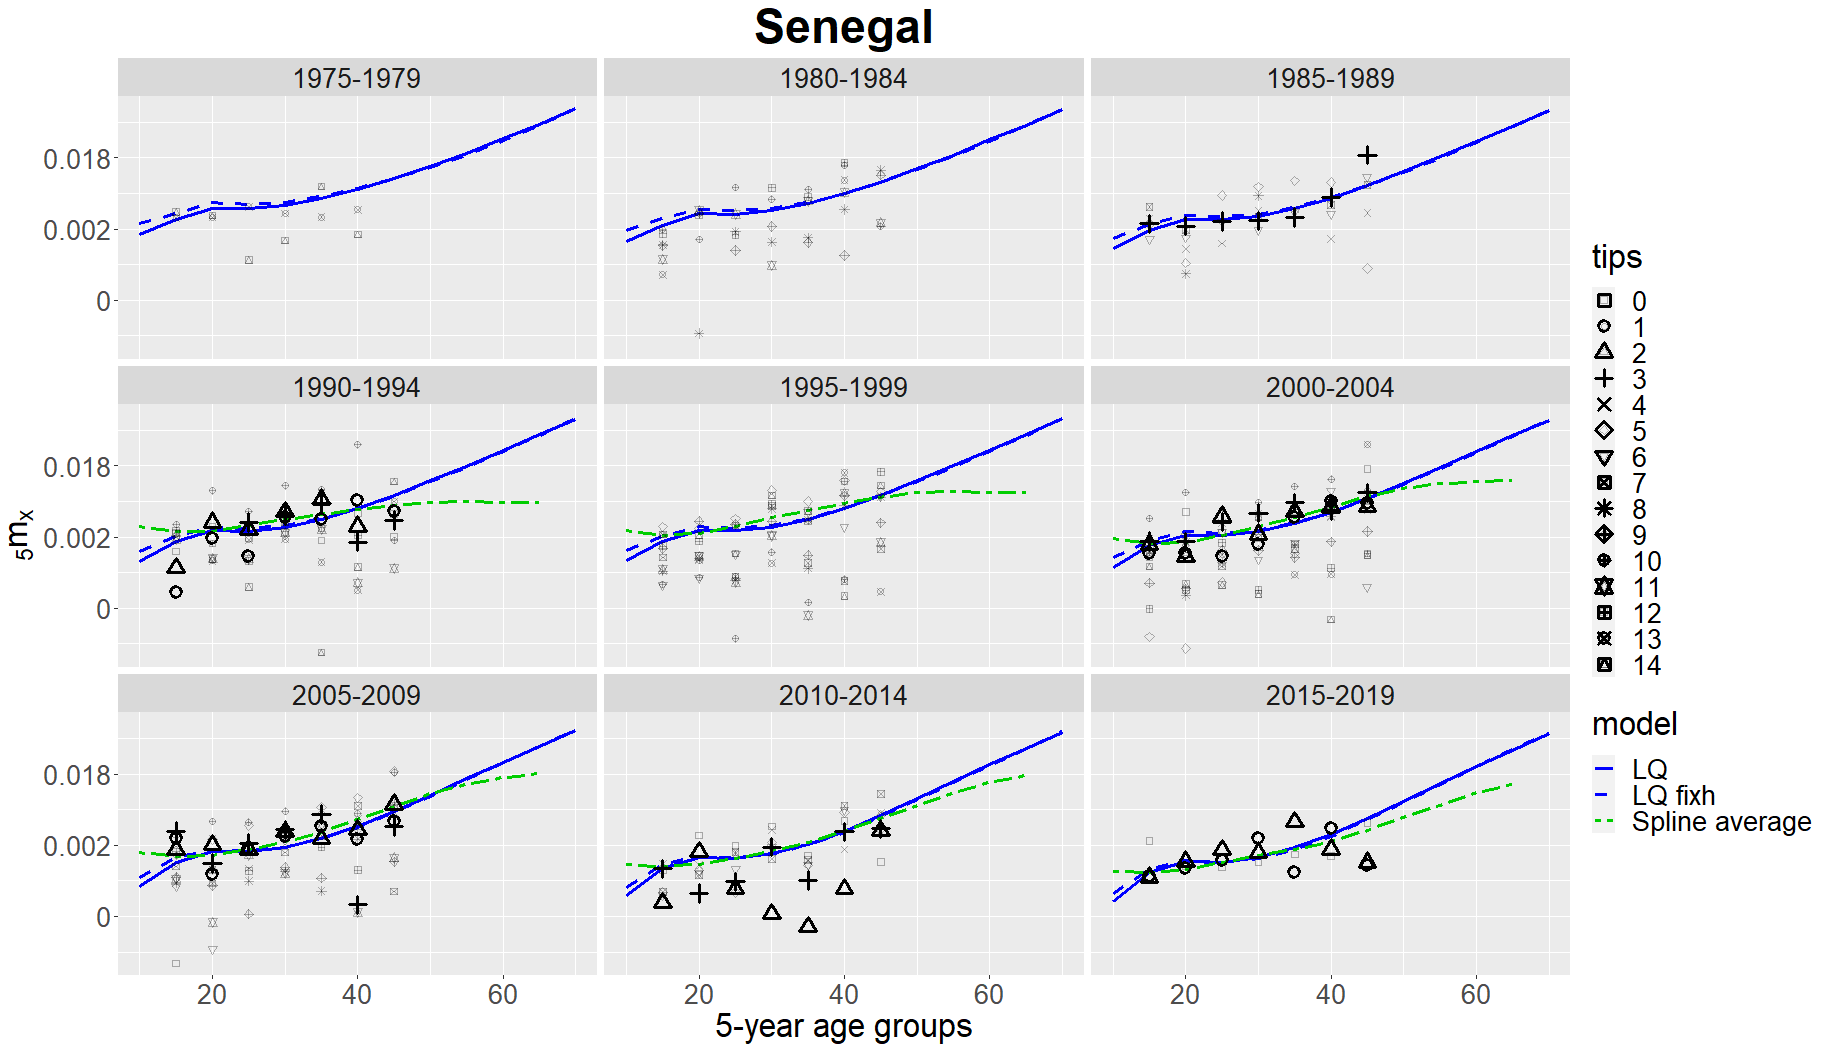
\includegraphics[width = \linewidth]{Burkina Faso/8/senegal males.png}
\end{figure}

\newpage
\section*{\centering Males}
\begin{figure}[H]
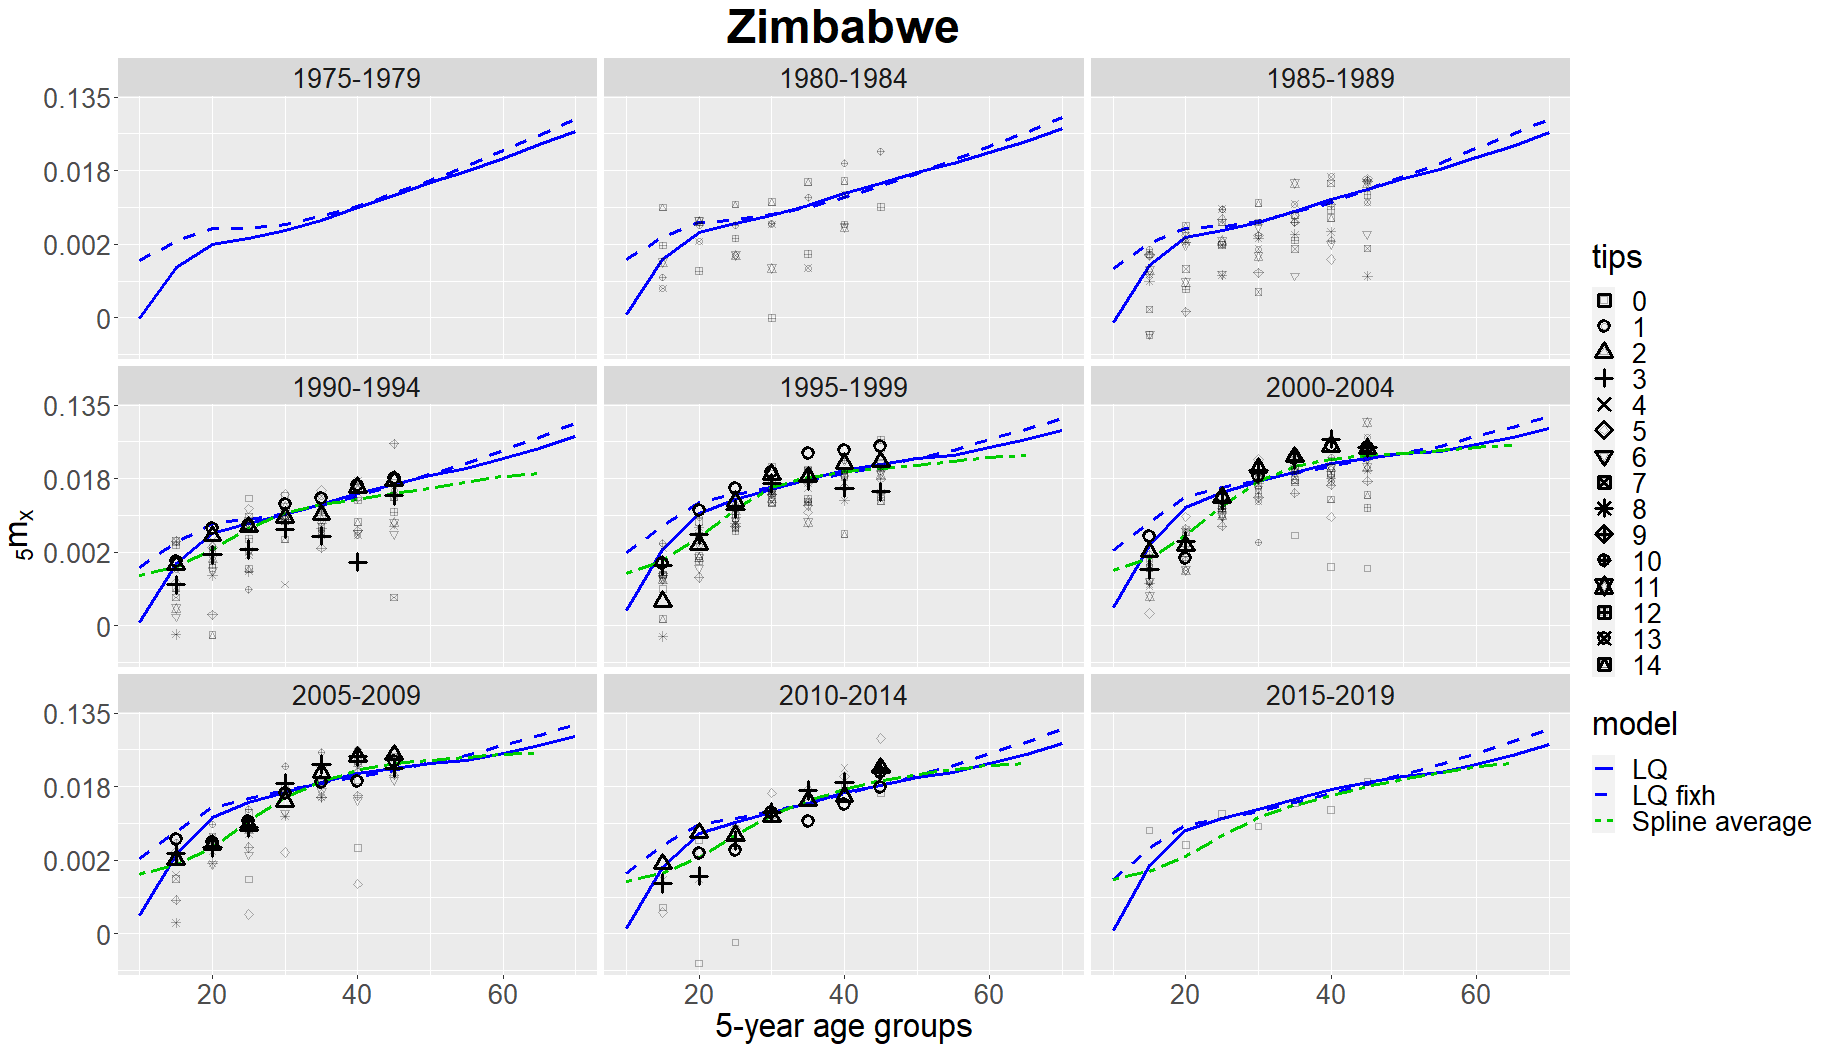
\includegraphics[width = \linewidth]{Burkina Faso/8/zimbabwe males.png}
\end{figure}
\begin{figure}[H]
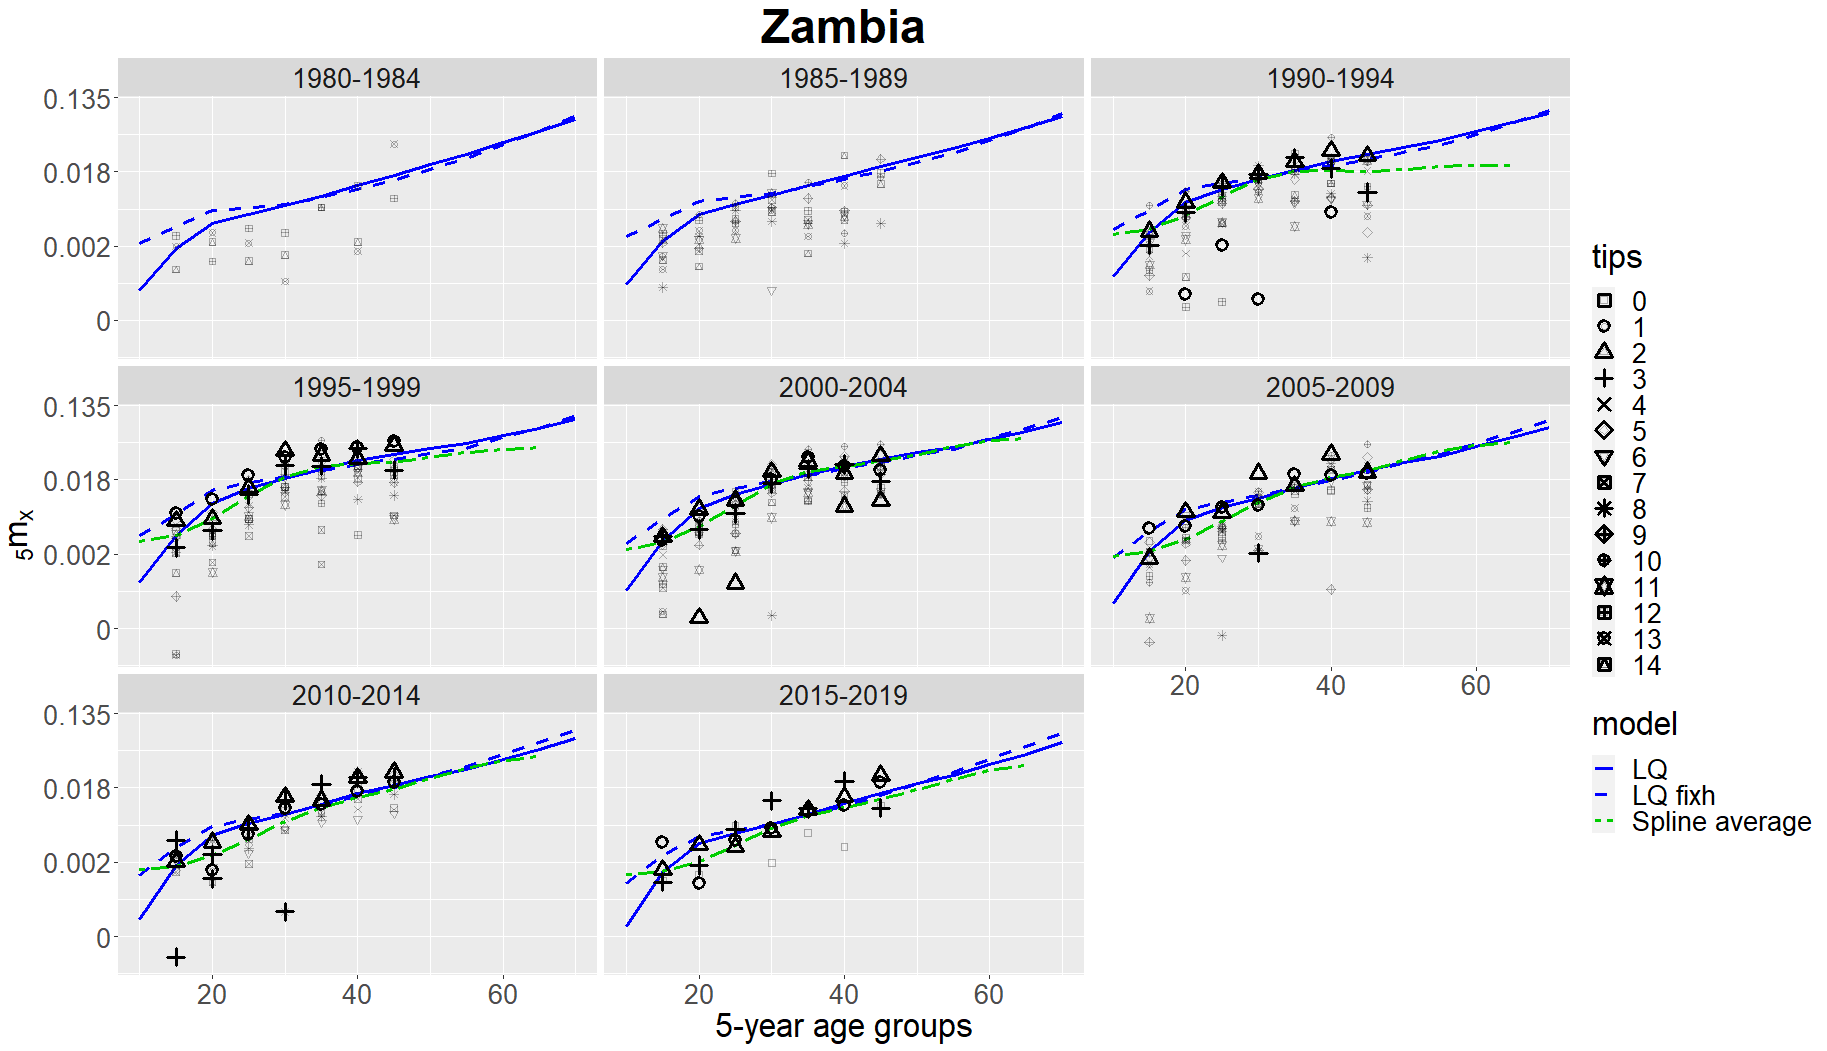
\includegraphics[width = \linewidth]{Burkina Faso/8/zambia males.png}
\end{figure}



\newpage
\section*{\centering Females}
\begin{figure}[H]
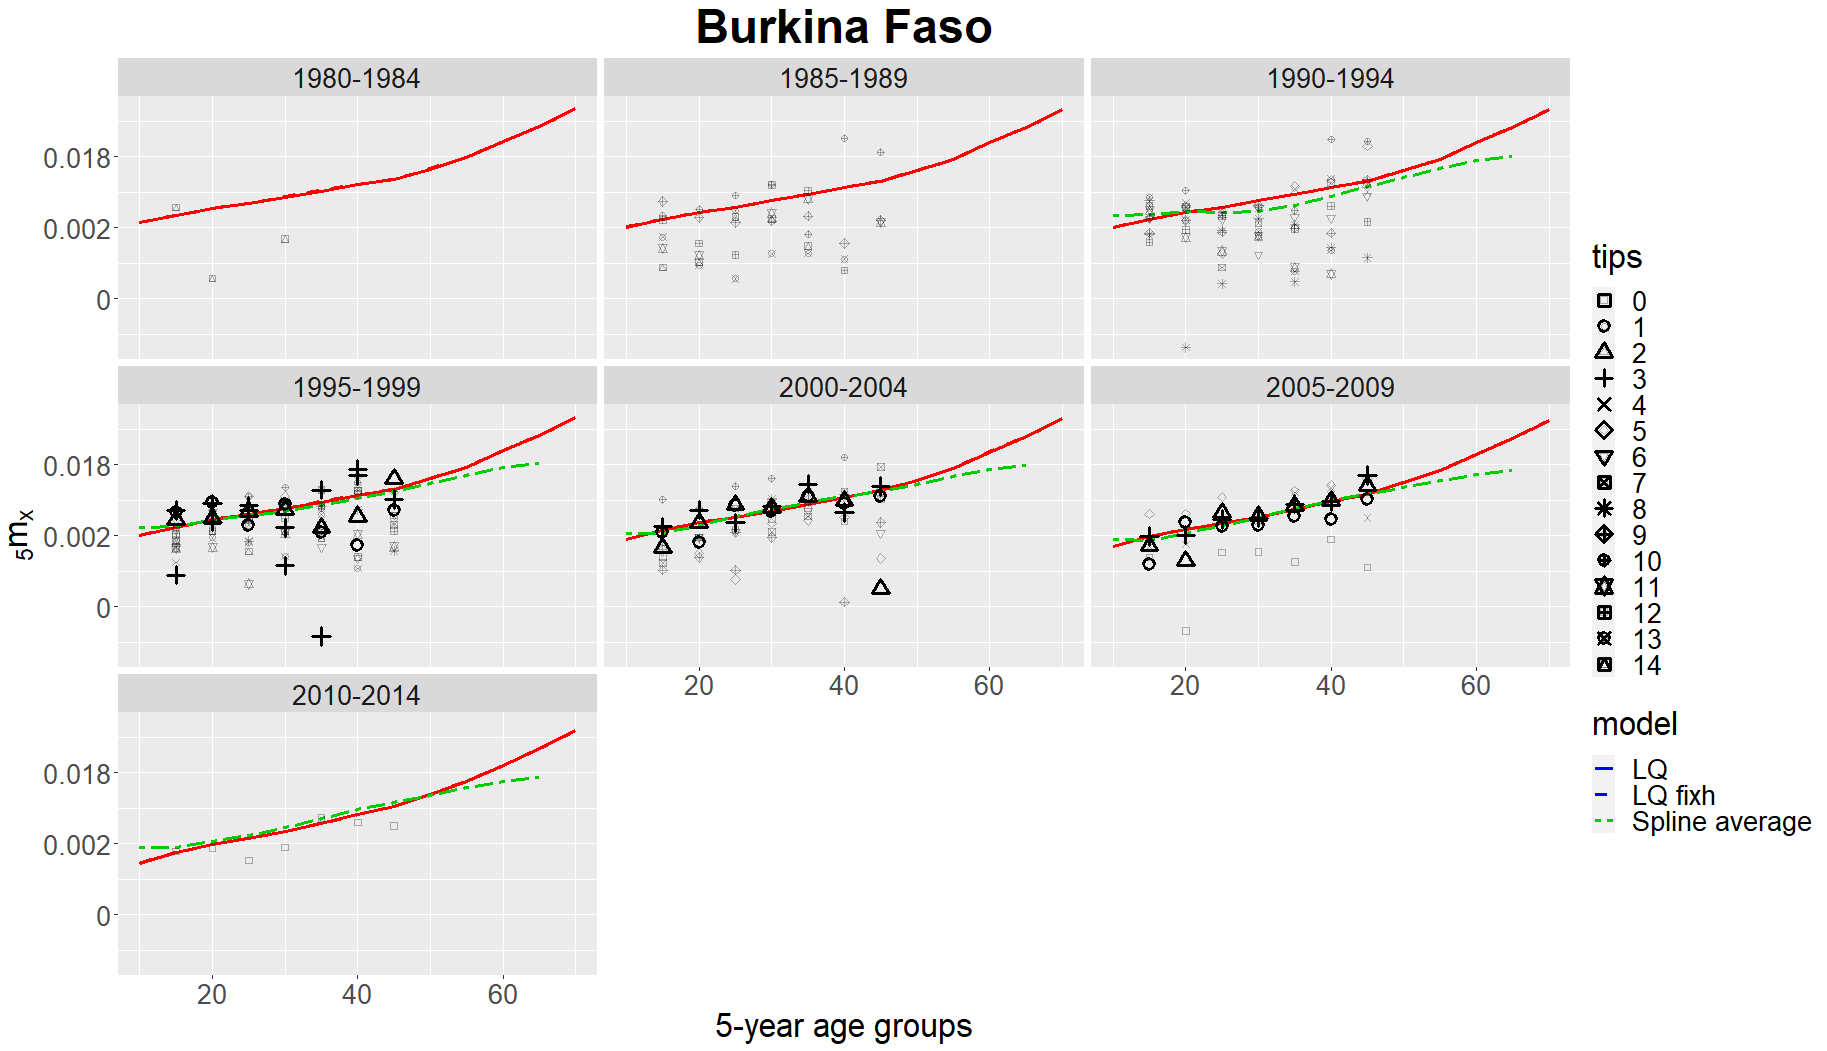
\includegraphics[width = \linewidth]{Burkina Faso/8/burkina faso females.png}
\end{figure}
\begin{figure}[H]
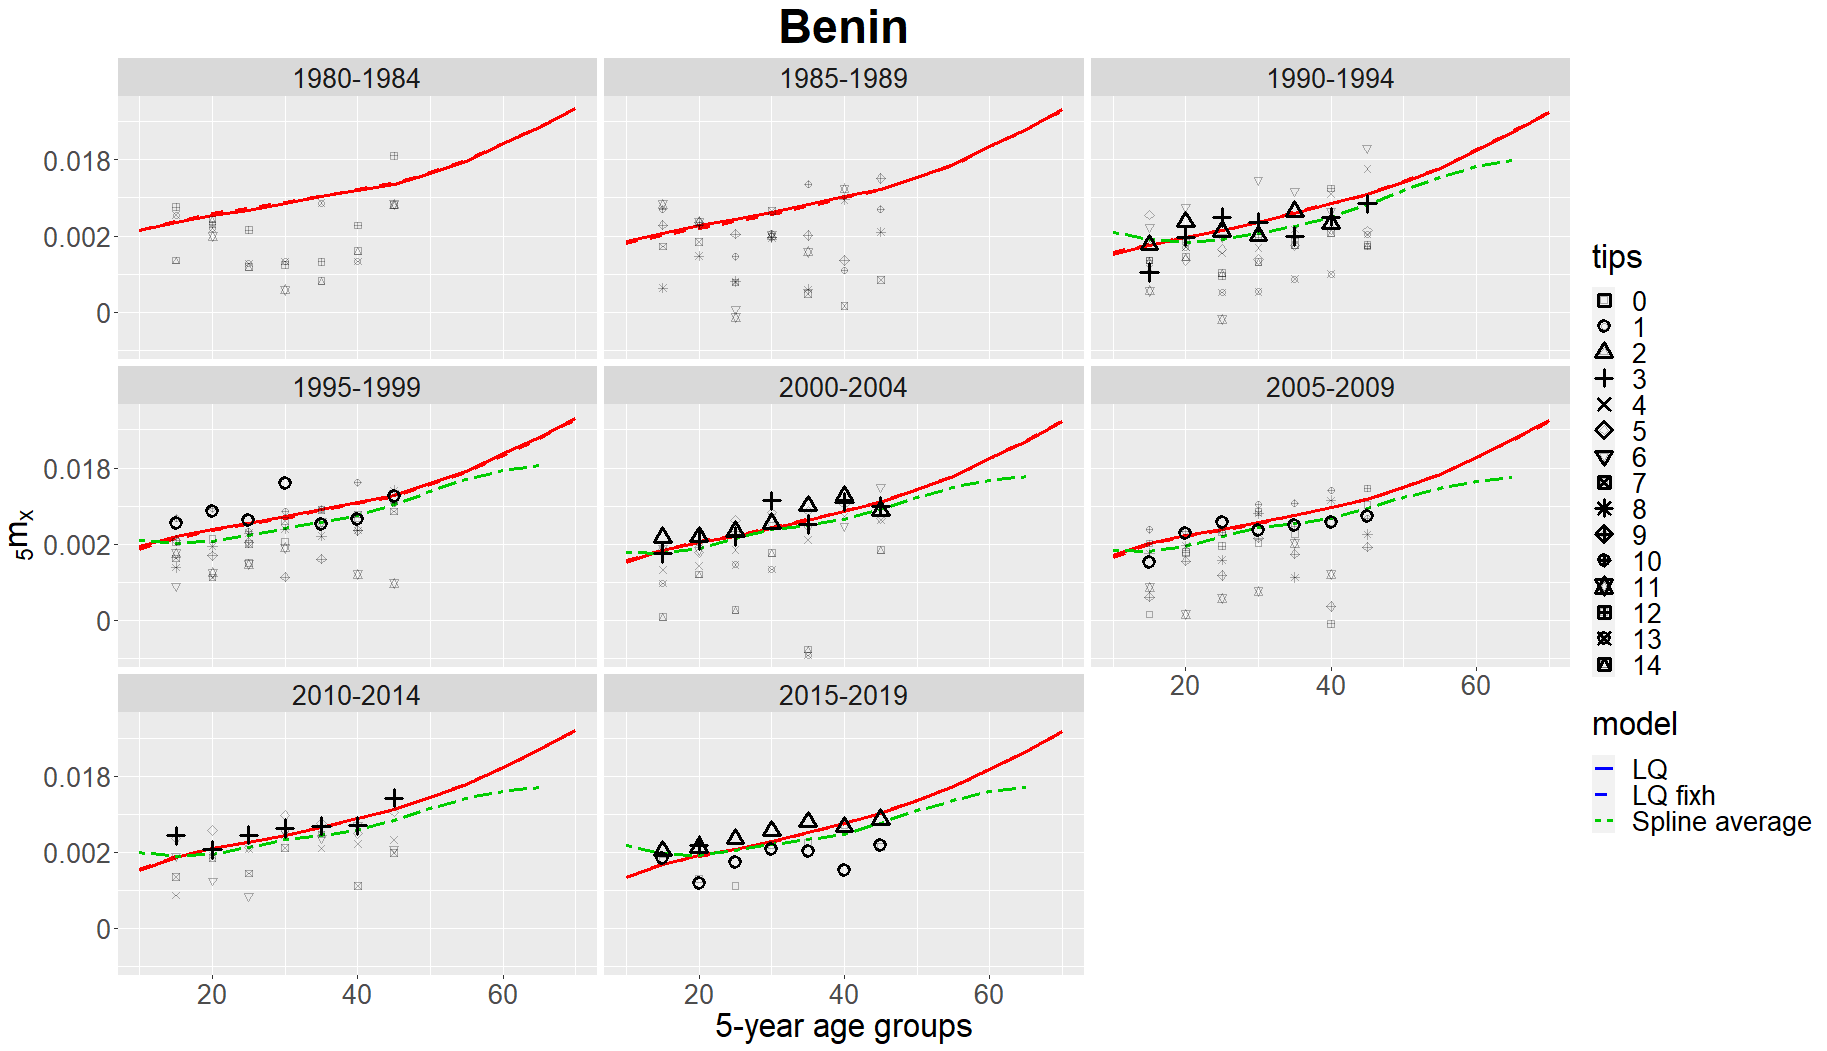
\includegraphics[width = \linewidth]{Burkina Faso/8/benin females.png}
\end{figure}

\newpage
\section*{\centering Females}
\begin{figure}[H]
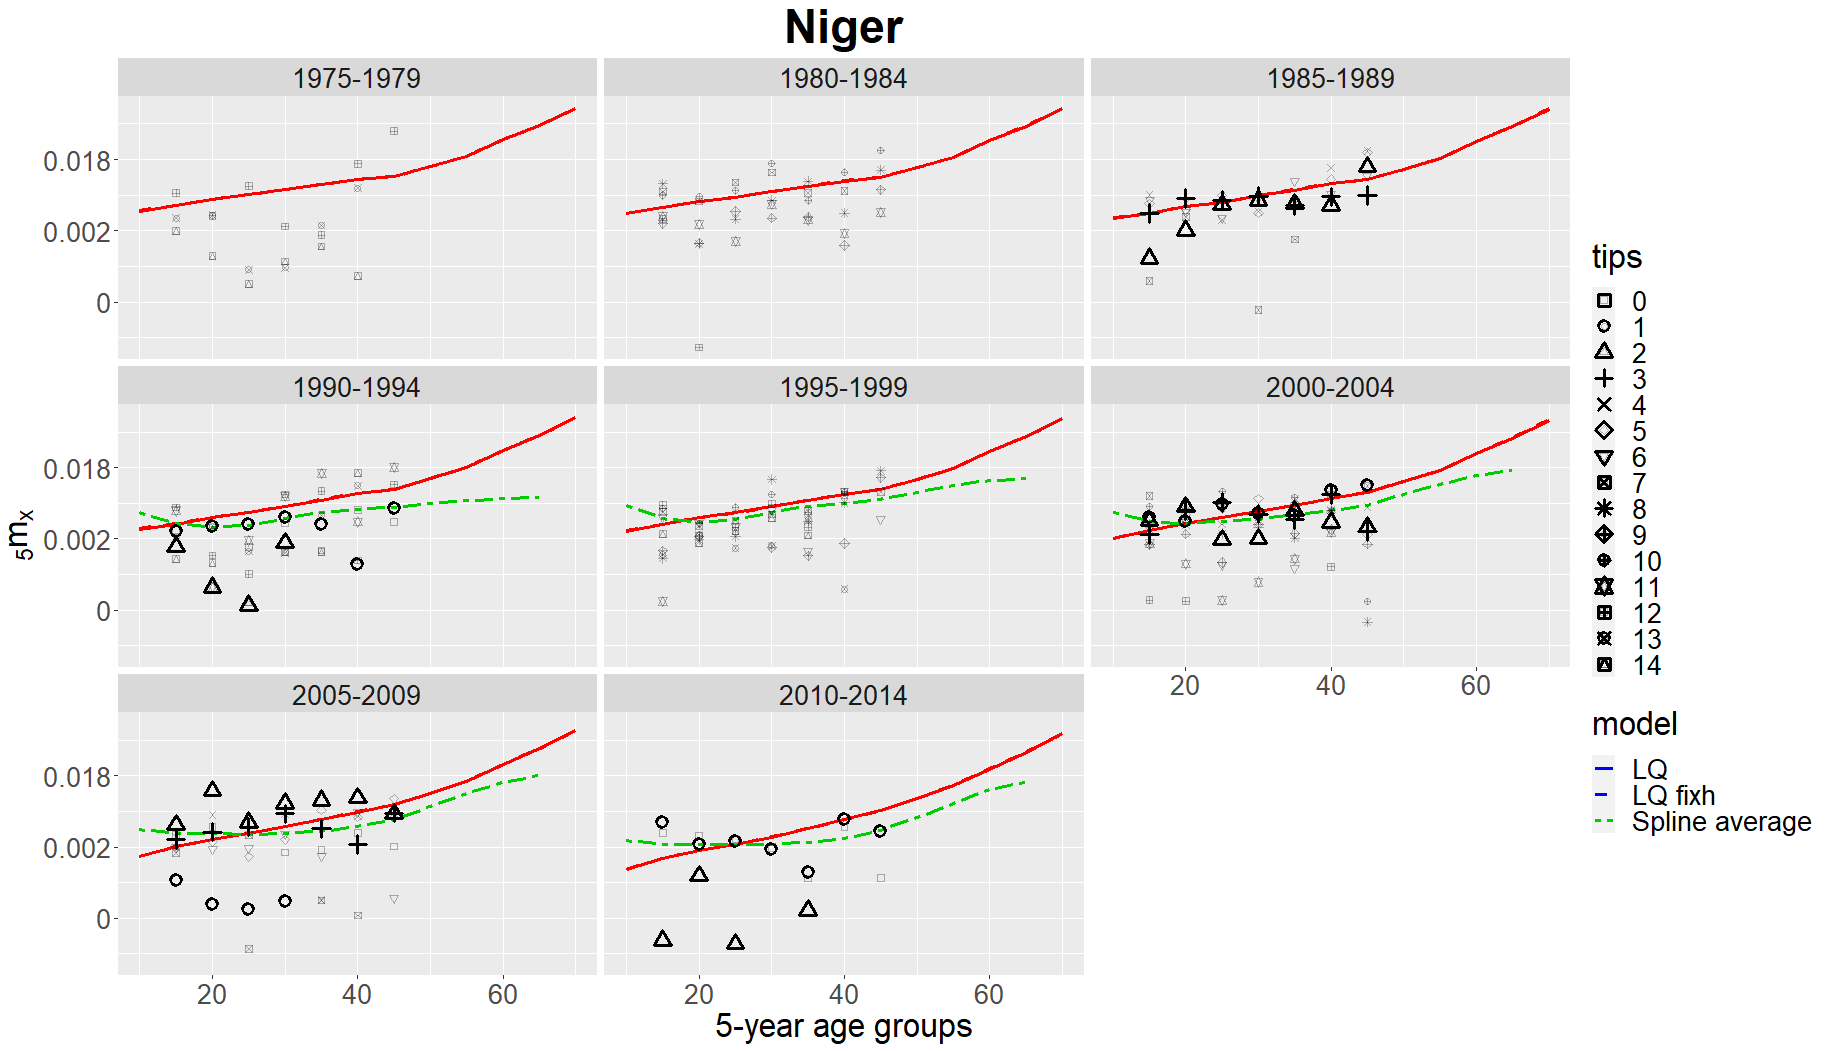
\includegraphics[width = \linewidth]{Burkina Faso/8/niger females.png}
\end{figure}
\begin{figure}[H]
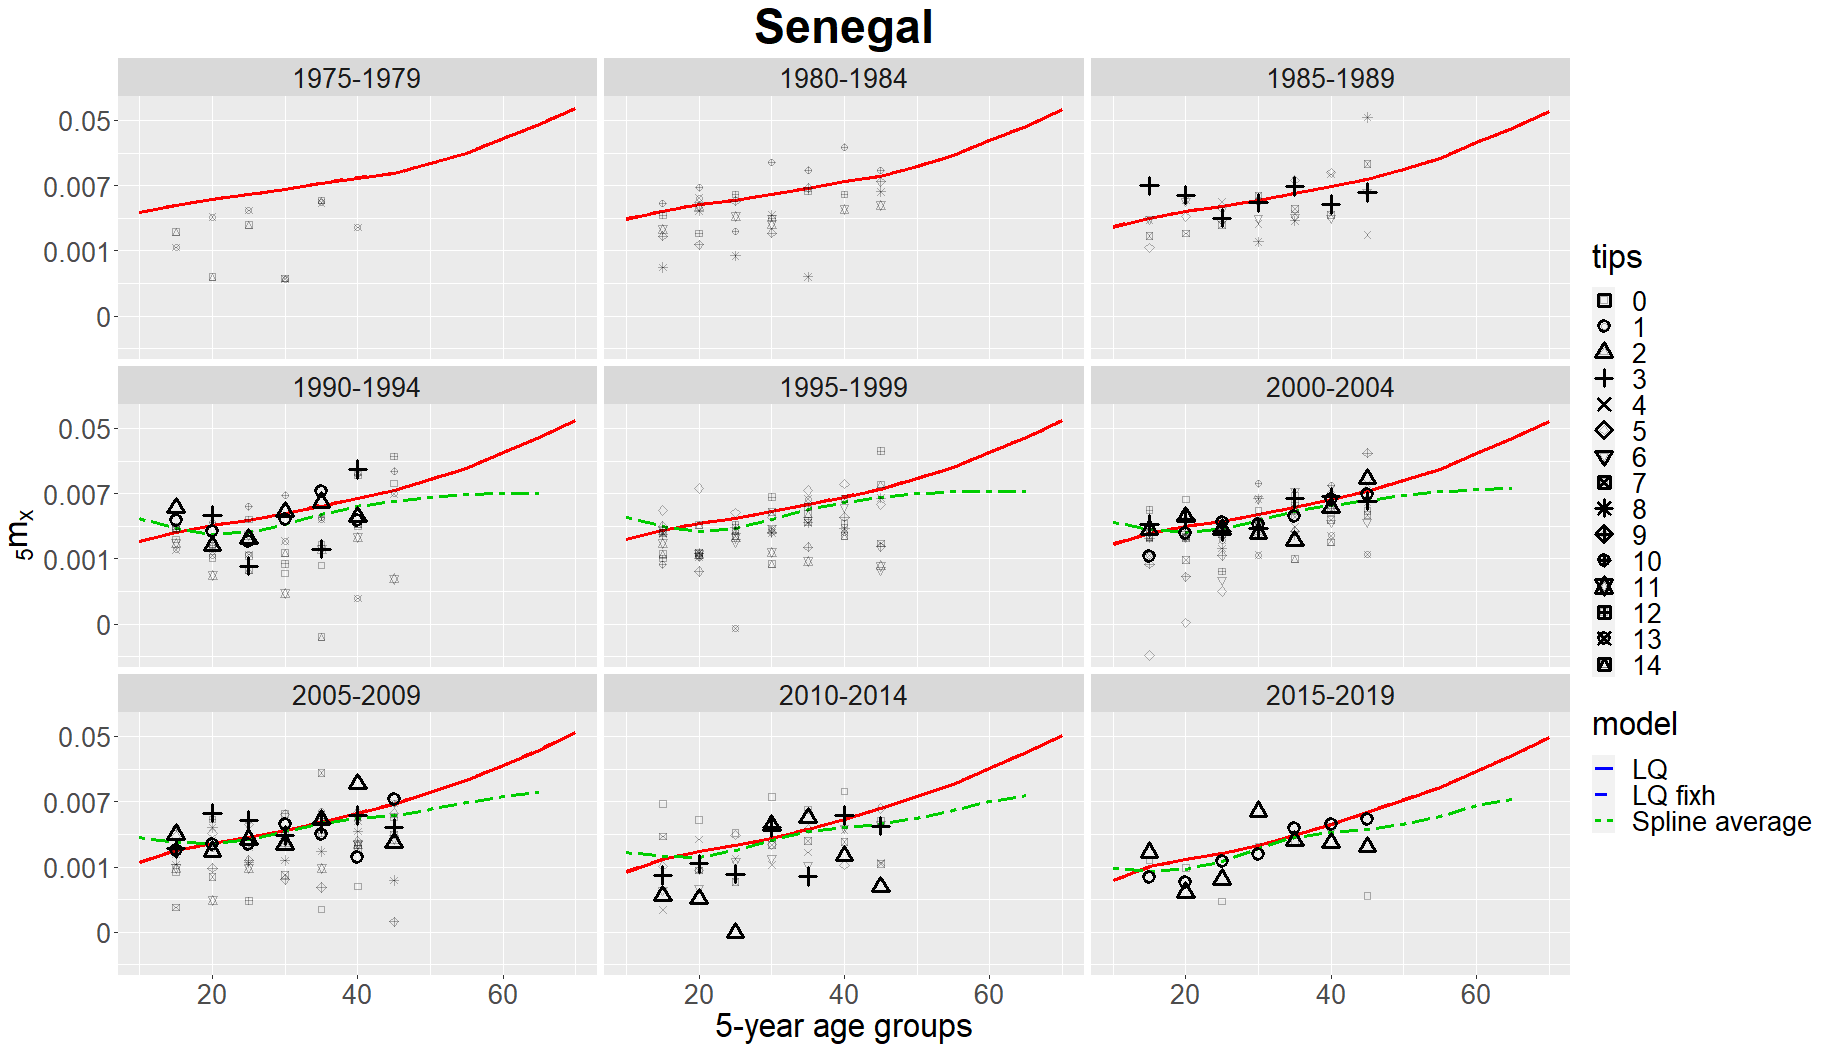
\includegraphics[width = \linewidth]{Burkina Faso/8/senegal females.png}
\end{figure}

\newpage
\section*{\centering Females}
\begin{figure}[H]
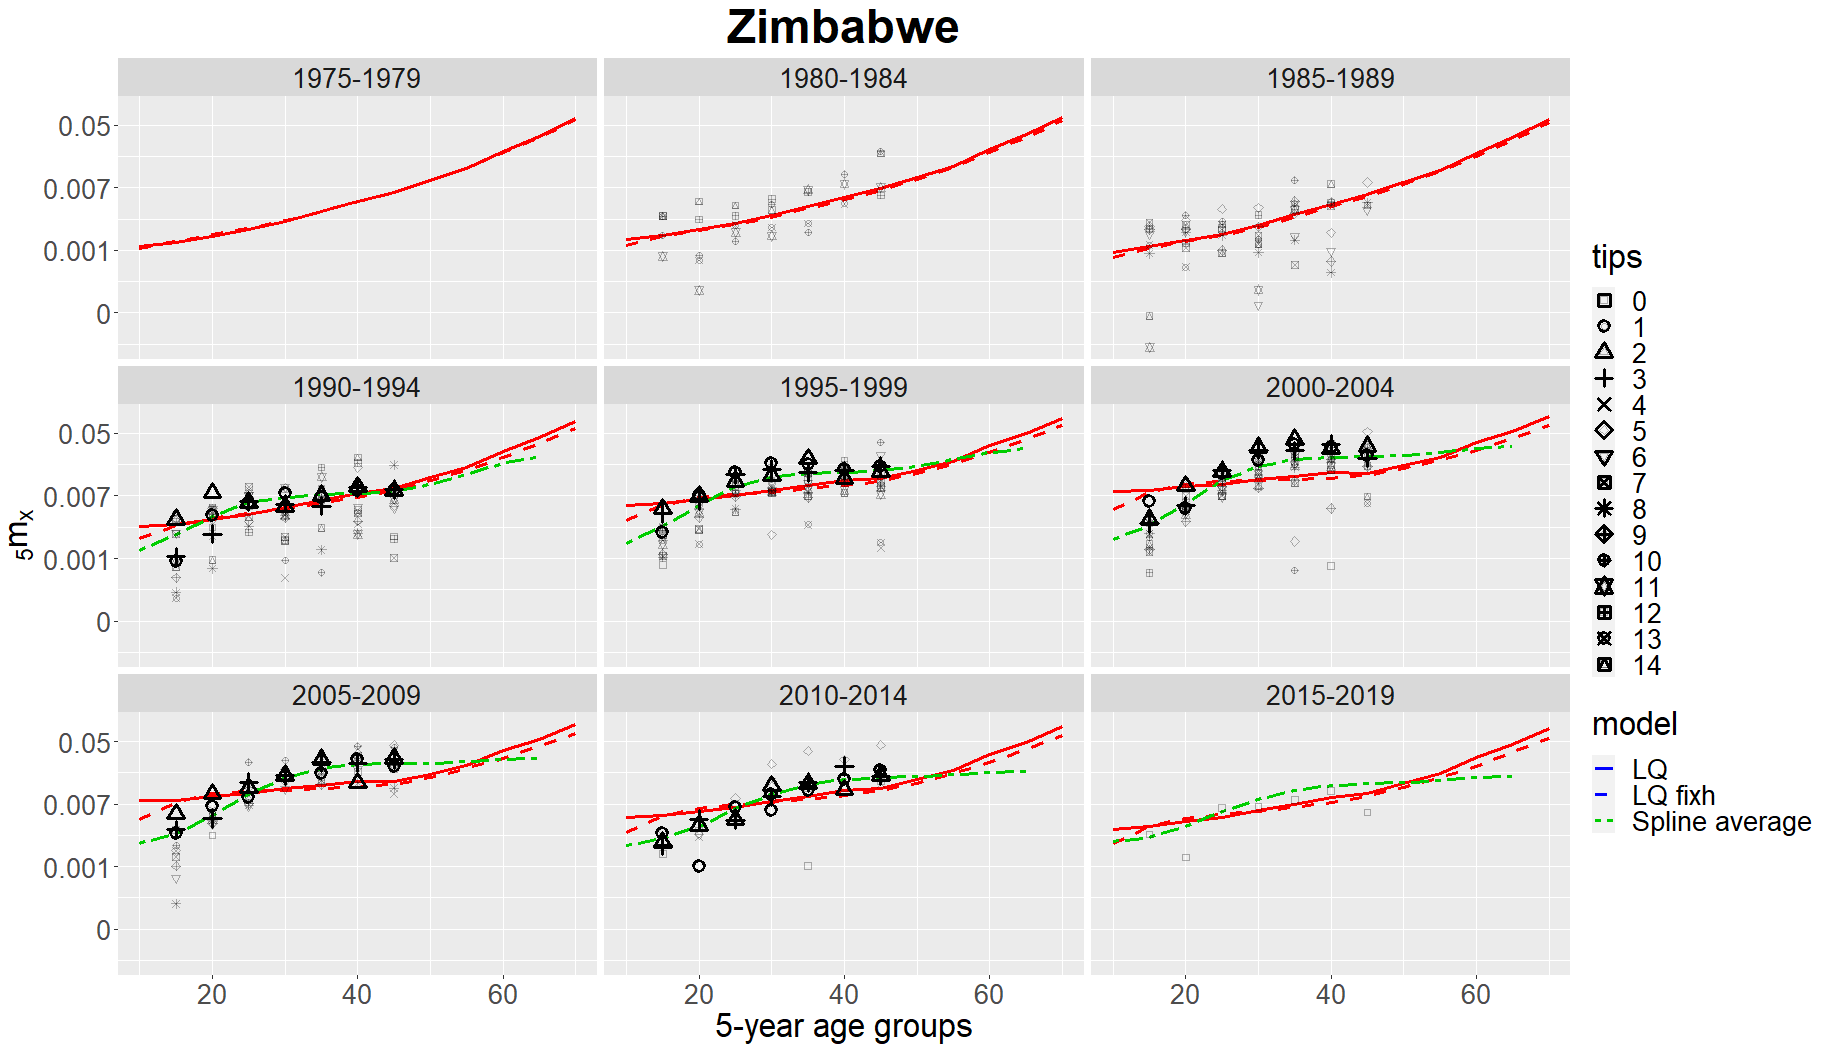
\includegraphics[width = \linewidth]{Burkina Faso/8/zimbabwe females.png}
\end{figure}
\begin{figure}[H]
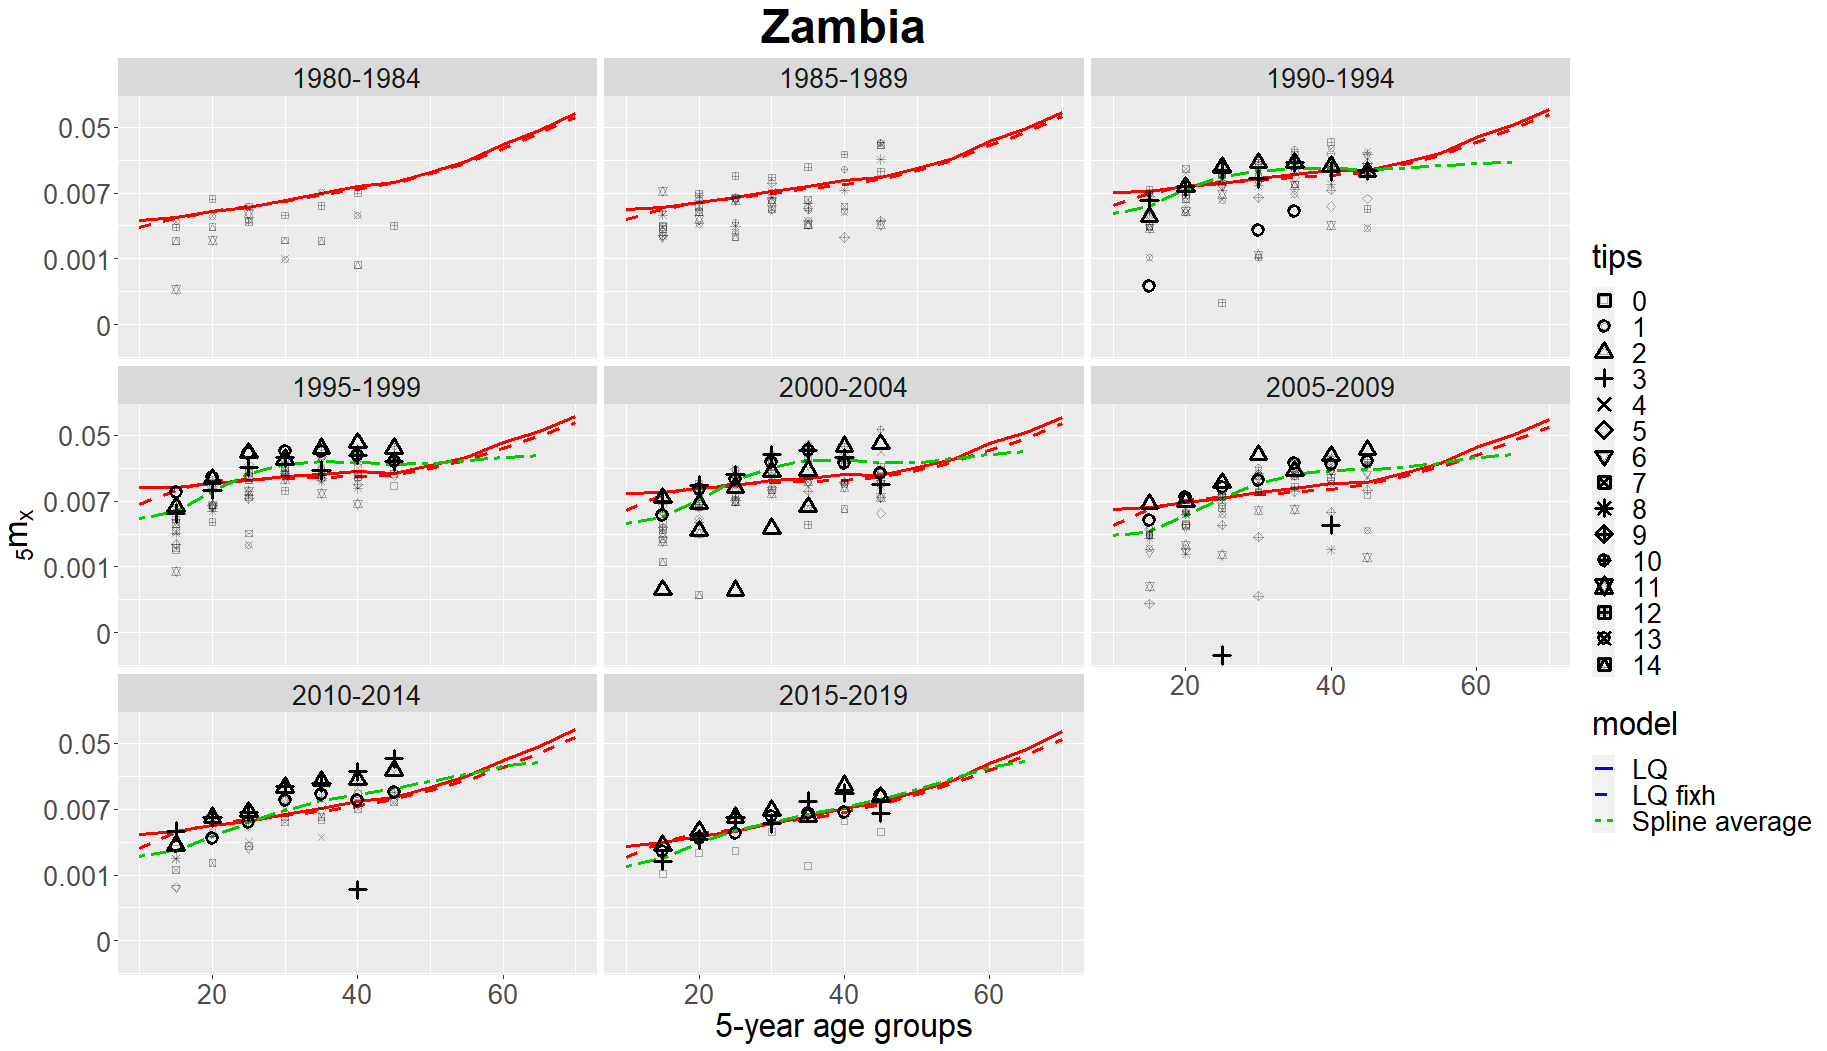
\includegraphics[width = \linewidth]{Burkina Faso/8/zambia females.png}
\end{figure}

\end{document} 